\chapter{TÍCH HỢP VÀ KẾT NỐI LIÊN SERVICE}

\section{Tổng quan về tích hợp trong Product A}

Một trong những yêu cầu quan trọng nhất của bài tập lớn là service không được tồn tại một mình. Mỗi service phải chứng minh được khả năng kết nối với ít nhất một service khác trong cùng Product. Đối với AI Vision Service, nhóm đã thiết lập kết nối với 3 service khác:

\begin{itemize}
    \item A2 - Camera Stream: kết nối đầu vào, AI Vision nhận ảnh từ Camera Stream.
    \item A6 - Core Business: kết nối đầu ra chính, AI Vision cung cấp kết quả phát hiện cho Core Business.
    \item A5 - Analytics: kết nối đầu ra phụ, AI Vision cung cấp detection log cho Analytics.
\end{itemize}

\section{Mô hình tích hợp}

\subsection{Phân biệt đồng bộ và bất đồng bộ}

\begin{table}[H]
\centering
\caption{So sánh giao tiếp đồng bộ và bất đồng bộ}
\label{tab:sync-async}
\ReportTableFont
\begin{tabular}{|>{\raggedright\arraybackslash}p{3cm}|>{\raggedright\arraybackslash}p{5cm}|>{\raggedright\arraybackslash}p{5cm}|}
\hline
\textbf{Tiêu chí} & \textbf{Đồng bộ (REST API)} & \textbf{Bất đồng bộ (Message Queue)} \\
\hline
Cơ chế & Request -> Response & Publish -> Subscribe \\
\hline
Độ trễ & Thấp, real-time & Có thể cao hơn \\
\hline
Coupling & Tight, caller chờ callee & Loose, decoupled \\
\hline
Độ tin cậy & Request fail nếu callee chết & Message có thể được lưu trong queue \\
\hline
Phù hợp & Cần kết quả ngay & Xử lý nền, broadcasting \\
\hline
\end{tabular}
\normalsize
\Nguon{Nhóm thực hiện}
\end{table}

AI Vision Service sử dụng REST API làm phương thức giao tiếp chính vì Camera Stream cần biết kết quả ngay để quyết định có gửi tiếp sang Core Business hay không.

\section{Kết nối A2 (Camera Stream) -> A4 (AI Vision)}

\subsection{Mô tả luồng kết nối}

\begin{enumerate}
    \item Camera IP liên tục ghi hình và gửi frame đến Camera Stream Service (A2).
    \item Camera Stream chạy motion detection. Khi phát hiện có chuyển động, nó tạo \Code{frame_url} và gọi \Code{POST /api/v1/vision/detect}.
    \item AI Vision tải ảnh, phân tích và trả về \Code{DetectionResult}.
    \item Camera Stream nhận kết quả và quyết định bước tiếp theo.
\end{enumerate}

\subsection{Hợp đồng API}

\begin{itemize}
    \item Endpoint: \Code{POST /api/v1/vision/detect}
    \item Method: POST
    \item Content-Type: application/json
    \item Request: \Code{VisionDetectRequest}
    \item Response 200: \Code{DetectionResult}
    \item Response 422: \Code{ProblemDetails} khi \Code{frame_url} không hợp lệ hoặc không tải được
\end{itemize}

\subsection{Phân tích độ tin cậy}

\begin{itemize}
    \item Timeout: \Code{httpx} client có timeout 15 giây.
    \item Retry: hiện chưa có cơ chế retry ở tầng API.
    \item Idempotency: mỗi request tạo một \Code{detection_id} mới, request giống hệt nhau gửi 2 lần vẫn tạo 2 detection khác nhau.
\end{itemize}

\section{Kết nối A4 (AI Vision) -> A6 (Core Business)}

\subsection{Vai trò của Core Business}

Core Business là "não trung tâm" của toàn bộ Product A. Nó nhận dữ liệu từ nhiều nguồn, áp dụng rule nghiệp vụ và ra quyết định. AI Vision cung cấp "mảnh ghép camera" cho Core Business.

\subsection{Adapter Pattern}

Nhóm implement Adapter Pattern để chuyển \Code{DetectionResult} sang \Code{CoreCameraEvent}.

\begin{table}[H]
\centering
\caption{Mapping giữa AI Vision và Core Business}
\label{tab:ai-core-mapping}
\ReportTableFont
\begin{tabular}{|>{\raggedright\arraybackslash}p{4cm}|>{\raggedright\arraybackslash}p{4cm}|>{\raggedright\arraybackslash}p{5cm}|}
\hline
\textbf{AI Vision} & \textbf{Core Business} & \textbf{Ghi chú} \\
\hline
\Code{detection_id} & \Code{event_id} & Giữ nguyên \\
\hline
\Code{anomaly_detected} & \Code{motion_detected} & Boolean tương đương \\
\hline
\Code{confidence_score} & \Code{motion_score} & Float 0-1 \\
\hline
\Code{person, conf >= 0.6} & \Code{unknown_person=true} & Phát hiện người lạ \\
\hline
\Code{risk_level} & \Code{risk_level} & Map 3 mức sang 3 mức \\
\hline
\end{tabular}
\normalsize
\Nguon{Nhóm thực hiện}
\end{table}

\subsection{Logic tự động ra quyết định}

AI Vision không chỉ trả về kết quả phân tích mà còn tự động đề xuất quyết định \Code{core_decision}. Điều này giúp Core Business không cần implement lại logic phân tích.

\begin{table}[H]
\centering
\caption{Ma trận quyết định của AI Vision}
\label{tab:decision-matrix}
\ReportTableFont
\begin{tabular}{|>{\raggedright\arraybackslash}p{3.9cm}|>{\raggedright\arraybackslash}p{2.0cm}|>{\raggedright\arraybackslash}p{3.1cm}|>{\raggedright\arraybackslash}p{4.0cm}|}
\hline
\textbf{Kịch bản} & \textbf{risk\_level} & \textbf{core\_decision} & \textbf{reason} \\
\hline
Không phát hiện gì & \TableCode{normal} & \TableCode{no_alert} & \TableCode{no_anomaly_detected} \\
\hline
Phát hiện người, conf $< 0.6$ & \TableCode{normal} & \TableCode{no_alert} & \TableCode{low_confidence_person} \\
\hline
Phát hiện người, conf $\geq 0.6$ & \TableCode{warning} & \TableCode{alert_required} & \TableCode{unknown_person_detected} \\
\hline
Phát hiện đối tượng, conf $< 0.85$ & \TableCode{warning} & \TableCode{alert_required} & \TableCode{object_detected} \\
\hline
Phát hiện đối tượng, conf $\geq 0.85$ & \TableCode{critical} & \TableCode{alert_required} & \TableCode{object_detected_high_conf} \\
\hline
\end{tabular}
\normalsize
\Nguon{Nhóm thực hiện}
\end{table}

\section{Kết nối A4 (AI Vision) -> A5 (Analytics)}

\subsection{Vai trò của Analytics}

Analytics tổng hợp dữ liệu từ nhiều nguồn để tạo báo cáo thống kê. AI Vision cung cấp detection log để Analytics phân tích theo camera, theo thời gian, theo loại đối tượng, theo mức rủi ro và theo model mode.

\subsection{Hợp đồng dữ liệu}

Các trường dữ liệu AI Vision cung cấp cho Analytics gồm:

\begin{itemize}
    \item \Code{detection_id}
    \item \Code{camera_id}
    \item \Code{timestamp}
    \item \Code{anomaly_detected}
    \item \Code{confidence_score}
    \item \Code{finding.object_name}
    \item \Code{finding.risk_level}
    \item \Code{model_mode}
\end{itemize}

\section{Luồng xử lý End-to-End}

\begin{sodo}[H]
    \centering
    \resizebox{0.96\textwidth}{!}{%
    \begin{tikzpicture}[
        font=\ReportDiagramFont,
        svc/.style={rectangle,draw=black,line width=0.8pt,minimum width=2.2cm,minimum height=0.82cm,align=center},
        store/.style={cylinder,shape border rotate=90,aspect=0.25,draw=black,line width=0.8pt,minimum width=1.6cm,minimum height=1.0cm,align=center},
        flow/.style={-{Latex[length=2.2mm]},line width=0.8pt},
        async/.style={-{Latex[length=2.2mm]},dashed,line width=0.8pt}
    ]
        \node[svc] (camera) at (0,2.1) {Camera IP};
        \node[svc] (stream) at (3.2,2.1) {A2\\Camera Stream};
        \node[svc] (vision) at (6.4,2.1) {A4\\AI Vision};
        \node[svc] (core) at (9.6,2.1) {A6\\Core Business};
        \node[svc] (notify) at (12.8,2.1) {A7\\Notification};

        \node[store] (analytics) at (6.4,-0.9) {A5\\Analytics};
        \node[svc,minimum width=2.8cm] (dashboard) at (9.6,-0.9) {Dashboard /\\Báo cáo};

        \draw[flow] (camera) -- node[midway,above,fill=white,inner sep=1pt]{frame} (stream);
        \draw[flow] (stream) -- node[midway,above,fill=white,inner sep=1pt]{URL} (vision);
        \draw[flow] (vision) -- node[midway,above,fill=white,inner sep=1pt]{event} (core);
        \draw[flow] (core) -- node[midway,above,fill=white,inner sep=1pt]{alert} (notify);

        \draw[async] (vision.south) -- node[midway,right,fill=white,inner sep=1pt]{detection log} (analytics.north);
        \draw[async] (core.south) -- node[midway,right,fill=white,inner sep=1pt]{decision log} (dashboard.north);
        \draw[flow] (analytics) -- node[midway,below,fill=white,inner sep=1pt]{metrics} (dashboard);
    \end{tikzpicture}
    }
    \SodoCaption{Luồng xử lý End-to-End trong Smart Campus Product A}{Nhóm thực hiện}
    \label{fig:end-to-end}
\end{sodo}

\section{Minh chứng giao diện và công cụ kiểm thử}

\begin{figure}[H]
\centering
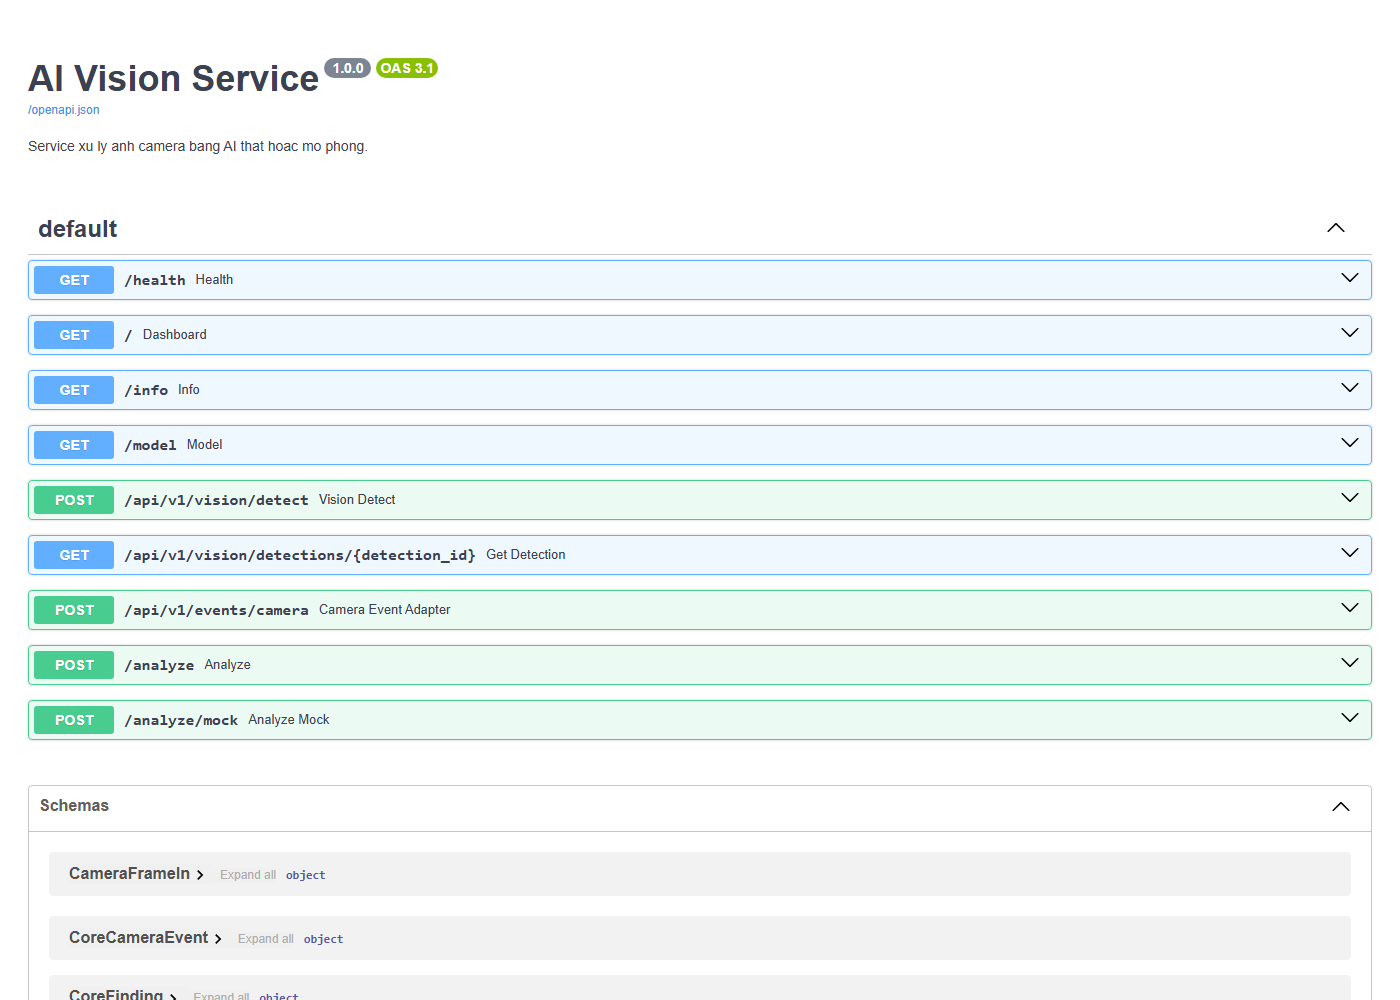
\includegraphics[width=0.96\textwidth]{images/swagger-ui.png}
\caption{Swagger UI -- Tài liệu API tự động của AI Vision Service}
\label{fig:swagger-ui}
\Nguon{Ảnh chụp từ giao diện Swagger UI của AI Vision Service}
\end{figure}

\begin{figure}[H]
\centering
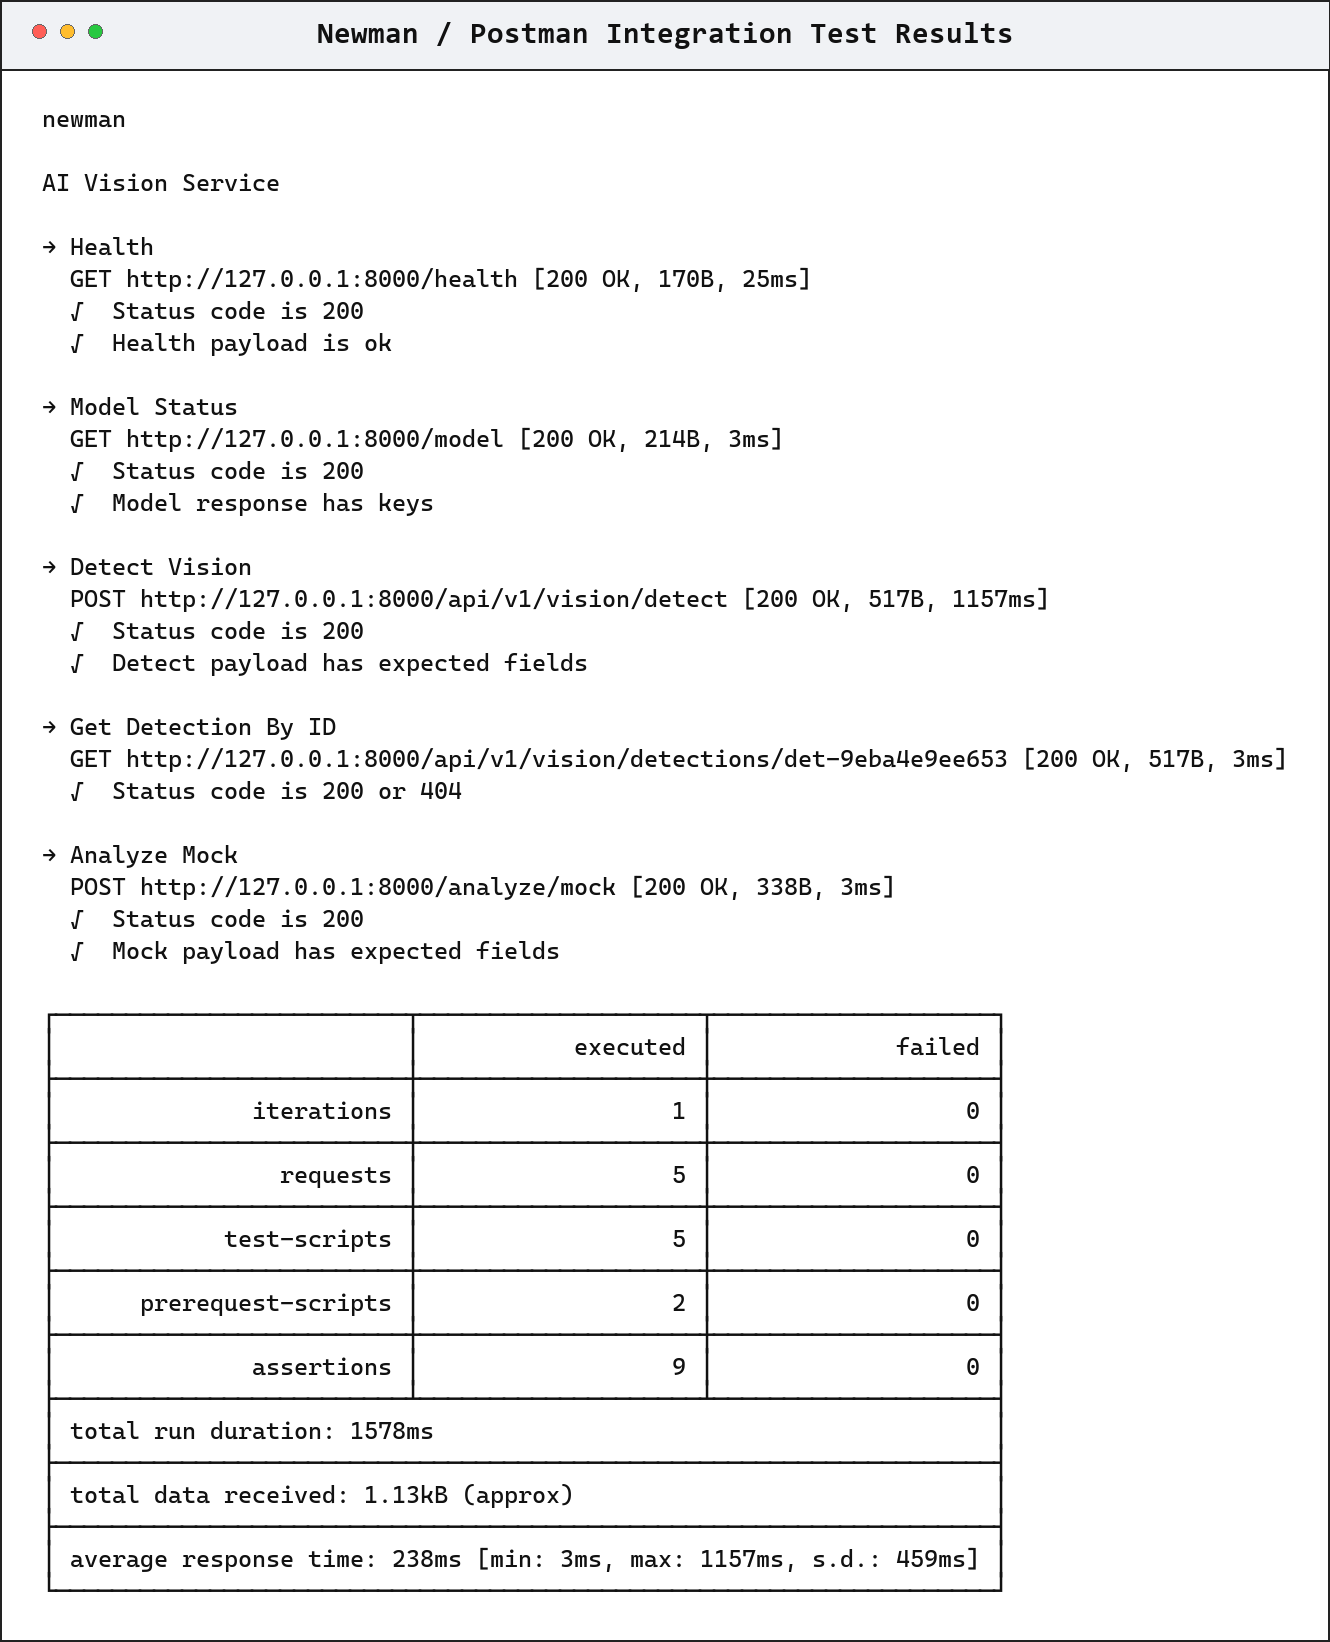
\includegraphics[width=0.96\textwidth]{images/postman-newman-results.png}
\caption{Postman -- Kết quả kiểm thử tích hợp}
\label{fig:postman-tests}
\Nguon{Kết quả chạy Postman collection bằng Newman}
\end{figure}

\begin{figure}[H]
\centering
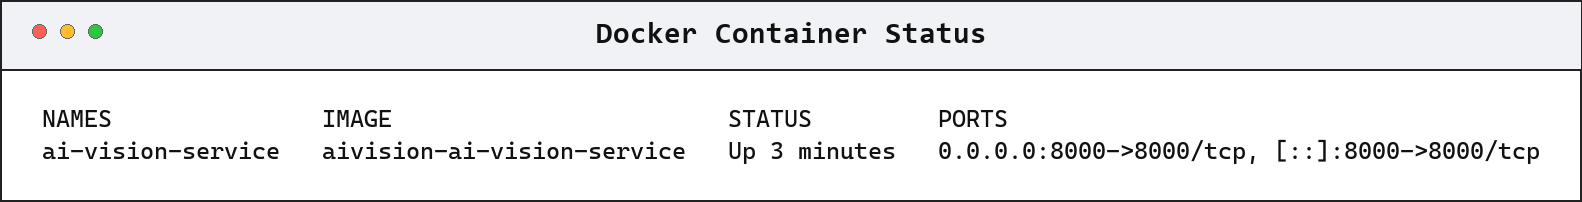
\includegraphics[width=0.96\textwidth]{images/docker-container-running.png}
\caption{Docker -- Container AI Vision Service đang hoạt động}
\label{fig:docker-running}
\Nguon{Kết quả thực tế từ lệnh \Code{docker ps}}
\end{figure}

\section{Tự đánh giá theo Rubric học phần}

\begin{table}[H]
\centering
\caption{Tự đánh giá chi tiết theo Rubric}
\label{tab:rubric}
\ReportTableFont
\begin{tabular}{|>{\raggedright\arraybackslash}p{3.6cm}|>{\raggedright\arraybackslash}p{1.8cm}|>{\raggedright\arraybackslash}p{2.2cm}|>{\raggedright\arraybackslash}p{5.8cm}|}
\hline
\textbf{Tiêu chí} & \textbf{Trọng số} & \textbf{Mức đạt} & \textbf{Minh chứng} \\
\hline
Service Boundary & 10\% & Tốt & Sơ đồ rõ, input/output/upstream/downstream đầy đủ \\
\hline
OpenAPI Contract & 20\% & Tốt & \Code{openapi.yaml}, schema, example, error model, Swagger UI \\
\hline
Testing & 15\% & Đạt & Postman 5 request, 9 assertion + smoke test, happy path, negative, error \\
\hline
Docker/Compose & 20\% & Tốt & Dockerfile + compose, chạy từ repo sạch, healthcheck \\
\hline
Integration & 20\% & Đạt & Kết nối A2, adapter cho A6, hợp đồng với A5 \\
\hline
Trình bày & 15\% & Tốt & \Code{PRESENTATION.md}, kịch bản 1 phút, thứ tự demo rõ ràng \\
\hline
\end{tabular}
\normalsize
\Nguon{Nhóm thực hiện}
\end{table}

\section{Phân công công việc}

\begin{table}[H]
\centering
\caption{Phân công công việc nhóm A4}
\label{tab:assignment}
\ReportTableFont
\begin{tabular}{|>{\raggedright\arraybackslash}p{3.5cm}|>{\raggedright\arraybackslash}p{2.8cm}|>{\raggedright\arraybackslash}p{5.7cm}|>{\centering\arraybackslash}p{1.4cm}|}
\hline
\textbf{Thành viên} & \textbf{Vai trò} & \textbf{Nhiệm vụ chính} & \textbf{Tỷ trọng} \\
\hline
\textbf{Trịnh Việt Đức} & Nhóm trưởng / Backend Lead & Điều phối nhóm, thiết kế kiến trúc, phát triển \Code{main.py}, \Code{vision.py}, xử lý ảnh, YOLO integration, làm việc với A2/A6/A5, tổng hợp nội dung báo cáo & 40\% \\
\hline
\textbf{Nguyễn Quang Đạt} & API/Contract Owner & Viết \Code{openapi.yaml}, Postman collection, smoke test, tài liệu API, hỗ trợ kiểm thử hợp đồng và minh chứng chạy thử & 30\% \\
\hline
\textbf{Lê Quang Dũng} & DevOps / Report & Docker, docker-compose, minh chứng vận hành, hỗ trợ tổng hợp báo cáo, phụ lục và kiểm tra bản dựng & 30\% \\
\hline
\end{tabular}
\normalsize
\Nguon{Nhóm thực hiện}
\end{table}

\subsection{Chữ ký xác nhận}

\begin{table}[H]
\centering
\begin{tabular}{|>{\centering\arraybackslash}p{4.8cm}|>{\centering\arraybackslash}p{4.8cm}|>{\centering\arraybackslash}p{4.8cm}|}
\hline
\textbf{Nguyễn Quang Đạt} & \textbf{Trịnh Việt Đức} & \textbf{Lê Quang Dũng} \\
\hline
\rule{0pt}{2.6cm} & \rule{0pt}{2.6cm} & \rule{0pt}{2.6cm} \\
\hline
\end{tabular}
\end{table}

\section{Hạn chế và hướng phát triển}

\subsection{Các điểm hạn chế hiện tại}

\begin{itemize}
    \item \Code{DETECTION_STORE} là Python dict trong RAM, mất toàn bộ dữ liệu khi restart.
    \item Giao tiếp hiện tại hoàn toàn đồng bộ qua REST API.
    \item YOLOv8n nhanh nhưng chưa mạnh ở các bài toán phức tạp.
    \item Chưa có xác thực, endpoint đang công khai.
    \item Dashboard còn đơn giản, chưa có real-time update.
\end{itemize}

\subsection{Hướng phát triển trong tương lai}

\begin{enumerate}
    \item Thay in-memory dict bằng PostgreSQL hoặc Redis.
    \item Tích hợp RabbitMQ hoặc Kafka cho giao tiếp bất đồng bộ.
    \item Nâng cấp AI lên YOLOv11 hoặc mô hình lớn hơn.
    \item Tích hợp nhận diện khuôn mặt.
    \item Thêm API key hoặc JWT authentication.
    \item Xây dashboard real-time bằng WebSocket.
    \item Chuyển sang Kubernetes.
    \item Thiết lập CI/CD bằng GitHub Actions.
\end{enumerate}

\section{Bảo mật và lưu trữ dữ liệu}

\subsection{Hiện trạng}

Hai hạn chế chính hiện tại là lưu trữ không bền vững và chưa có xác thực.

\subsection{Giải pháp đề xuất}

\begin{enumerate}
    \item Thay thế in-memory store bằng PostgreSQL.
    \item Thêm JWT authentication.
    \item Sử dụng API key cho service-to-service.
\end{enumerate}

\subsection{So sánh các phương án}

\begin{table}[H]
\centering
\caption{So sánh phương án lưu trữ và xác thực}
\label{tab:security-options}
\ReportTableFont
\begin{tabular}{|>{\raggedright\arraybackslash}p{3cm}|>{\raggedright\arraybackslash}p{3.2cm}|>{\raggedright\arraybackslash}p{3.2cm}|>{\raggedright\arraybackslash}p{3.2cm}|}
\hline
\textbf{Tiêu chí} & \textbf{Hiện tại} & \textbf{PostgreSQL + JWT} & \textbf{Redis + API Key} \\
\hline
Lưu trữ & In-memory & Bền vững & Bền vững \\
\hline
Tốc độ & Nhanh nhất & Trung bình & Nhanh \\
\hline
Phức tạp & Đơn giản nhất & Trung bình & Đơn giản \\
\hline
Xác thực & Không có & JWT & API Key \\
\hline
Phù hợp & Demo & Production & Production nhẹ \\
\hline
\end{tabular}
\normalsize
\Nguon{Nhóm thực hiện}
\end{table}

\section{Kết luận chương}

Chương này đã trình bày kết nối của AI Vision với A2, A6, A5, mô hình tích hợp, adapter pattern, ma trận quyết định, luồng end-to-end, tự đánh giá theo rubric, phân công công việc, hạn chế và hướng phát triển.

